\subsection{Schedule generation}
\begin{figure}[H]\centering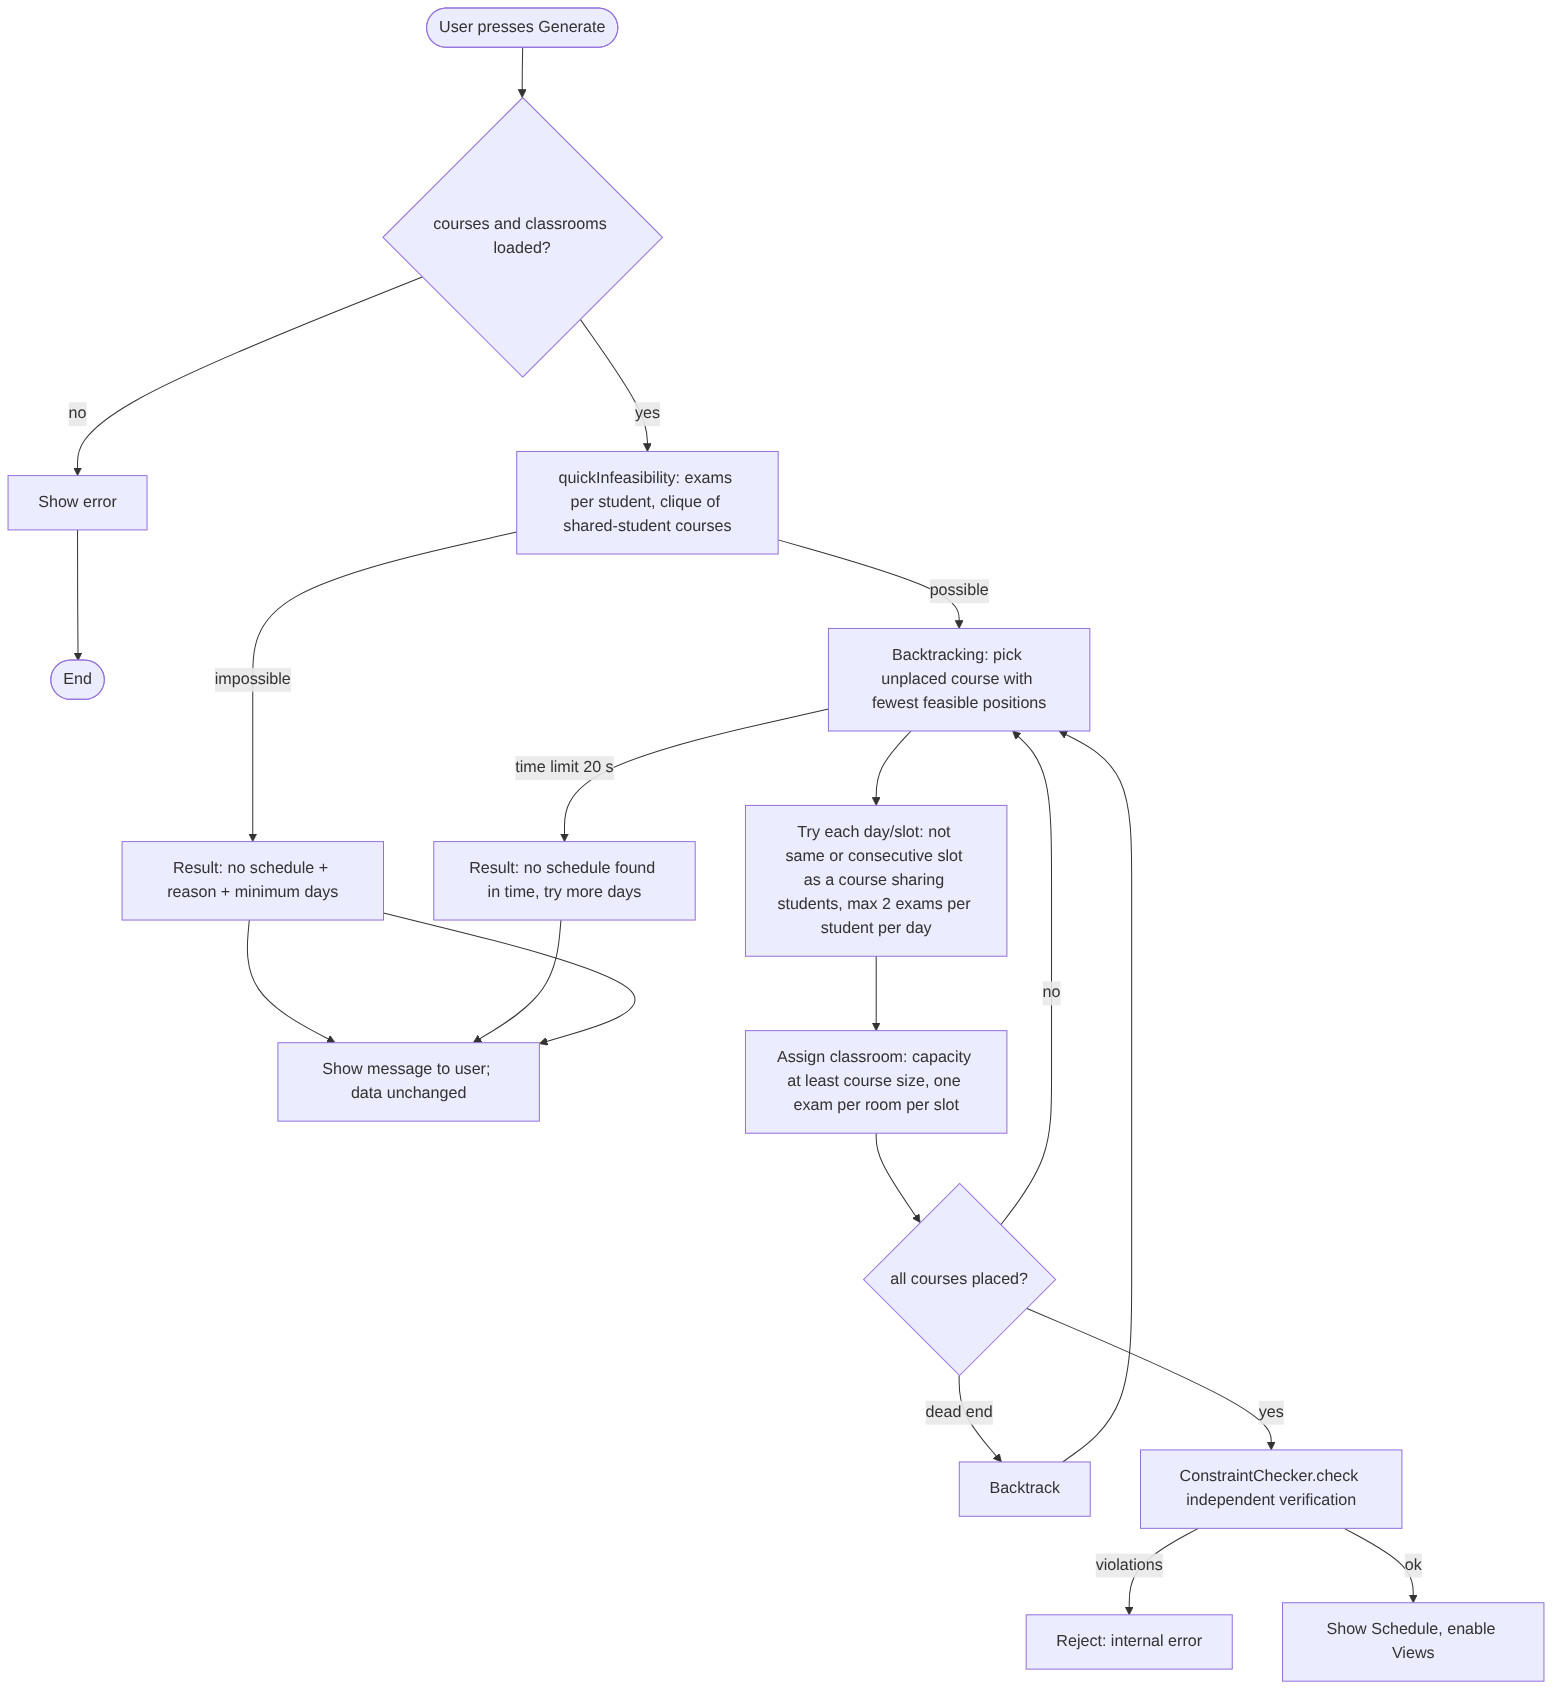
\includegraphics[width=0.75\textwidth]{figures/generate_flow.png}\caption{Schedule generation.}\end{figure}
The algorithm is a backtracking search. At each step it selects the unplaced course that has the fewest feasible positions (day, slot) left, tries those positions and assigns a classroom whose capacity is at least the course size and that is free in that slot; if no position works it backtracks. A position is feasible when no course sharing a student is in the same or an adjacent slot of that day and no student would have more than two exams that day. The search stops after 20 seconds. Before the search a quick check rules out obviously impossible periods (Section~3.3). A found schedule is verified by the independent \texttt{ConstraintChecker} before it is shown. Optional goals: \emph{fewest days} tries 1, 2, \dots days and keeps the first period that works; \emph{spread evenly} balances exams over the available days.
